\usetikzlibrary{positioning,shapes,shadows,arrows,calc}
\tikzstyle{role}=[rectangle, draw=black, rounded corners, fill=white, drop shadow,
        text centered, anchor=north, text=black, text width=3cm]
\tikzstyle{class}=[rectangle, draw=black, fill=white, drop shadow,
        text centered, anchor=north, text=black, text width=3cm]
\tikzstyle{inheritance}=[->, >=open triangle 90, thick]
\tikzstyle{line}=[-, thick]

\begin{figure}[t!]
\begin{center}
\TUFont

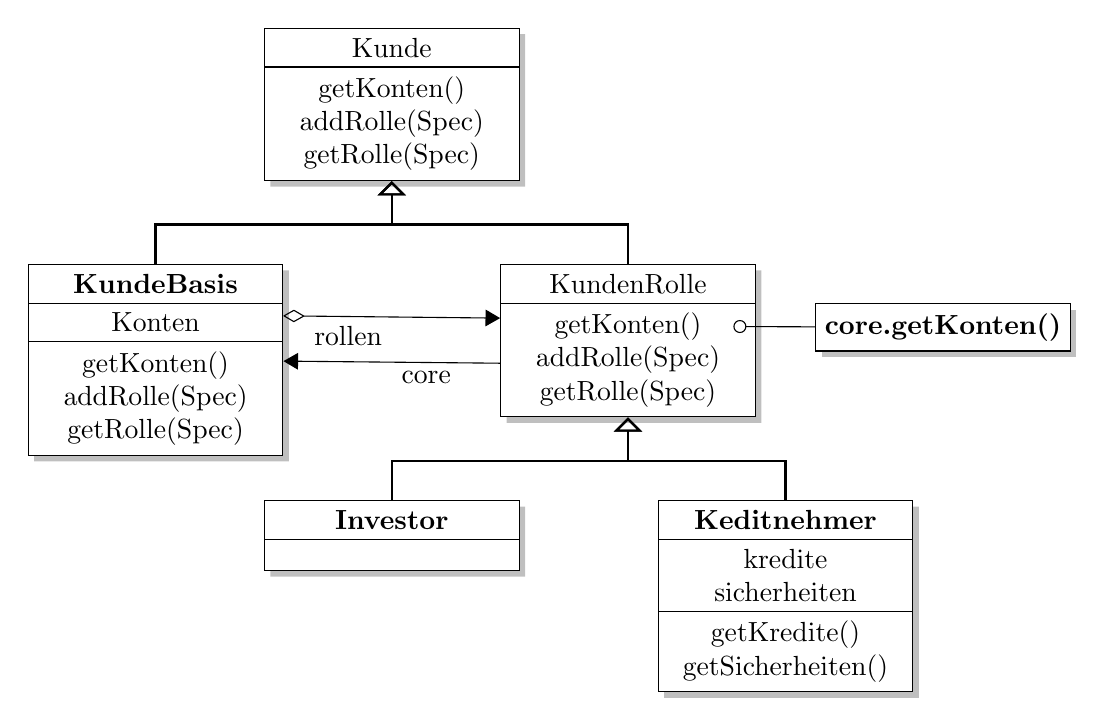
\begin{tikzpicture}[node distance=1.0cm]
     	   		    \node (Kunde) [class, rectangle split, rectangle split parts=2]
     	   		        {
     	   		            \textbfit{Kunde}
     	   		            \nodepart{second}getKonten()\\addRolle(Spec)\\getRolle(Spec)
     	   		        };
     	   		    \node [class, rectangle split, rectangle split parts=3] (CustomerNatural) at (-3,-3) {
     	   		            \textbf{KundeBasis}
     	   		            \nodepart{second}Konten
     	   		            \nodepart{third}getKonten()\\addRolle(Spec)\\getRolle(Spec)
     	   		            
     	   		        };
     	   		    \node [class, rectangle split, rectangle split parts=2] (KundeRole) at (3,-3) {
     	   		            \textbfit{KundenRolle}
     	   		            \nodepart{second}getKonten()\\addRolle(Spec)\\getRolle(Spec)
     	   		        };
     	   		    %\node (AuxNode02) [text width=0.5cm, below=of KundeRole] {};
     	   		    \node [class, rectangle split, rectangle split parts=2] (Investor) at (0,-6) {
     	   		            \textbf{Investor}
     	   		        };
     	   		    \node [class, rectangle split, rectangle split parts=3] (Borrower) at (5,-6) {
     	   		            \textbf{Keditnehmer}
     	   		            \nodepart{second}kredite\\sicherheiten
     	   		            \nodepart{third}getKredite()\\getSicherheiten()
     	   		        };
     	   		         \node [class, rectangle split, rectangle split parts=1] (Comment) at (7,-3.5) {
     	   		            \textbf{core.getKonten()}
     	   		        };     
     	   		    
     	   		    %\draw[line] (CustomerNatural.north) -- ++(0,0.5) -| (Kunde.south);
     	   		    \draw[inheritance] (CustomerNatural.north) -- ++(0,0.5) -| (Kunde.south);
     	   		    
     	   		    
     	   		    \draw[inheritance] (KundeRole.north) -- ++(0,0.5) -| (Kunde.south);
     	   		    %\draw[line] (KundeRole.north) -- ++(0,0.5) -| (Kunde.south);
     	   		    
     	   		    \draw[inheritance] (Investor.north) -- ++(0,0.5) -| (KundeRole.south);
     	   		    %\draw[line] (Investor.north) -- ++(0,0.5) -| (KundeRole.south);
     	   		    
     	   		    \draw[inheritance] (Borrower.north) -- ++(0,0.5) -| (KundeRole.south);
     	   		    %\draw[line] (Borrower.north) -- ++(0,0.5) -| (KundeRole.south);     	   		    
     	   		        \node (anchor) at (4.2139,-3.7945) {};
     	   		        
     	   		\draw[open diamond-triangle 60]  (CustomerNatural.19) -- node[below left]{rollen} (KundeRole.170);
     	   		\draw[triangle 60-]  (CustomerNatural) -- node[below right]{core} (KundeRole.190);

			\draw [-o] (Comment) edge (anchor);

\end{tikzpicture}
\caption[Das Role-Object Pattern an einem Beispiel]{Klassendiagramm mit Role-Object Pattern am Beispiel einer Kundenhierarchie einer Bank nach \cite{baumer1998role}}
\label{fig:roleobjectbsp}
\end{center}
\end{figure}

